\documentclass{../../td}
\begin{document}
\subsection*{Exercice 1}
\begin{enumerate}
\item Pour trouver les points d'équilibres, on annuler les dérivées des positions:
\[
\left \{ \begin{matrix}
0 = \sigma(x_2-x_1)\\
0 = \rho x_1 - x_2-x_1x_3\\
0 = -\beta x_3 + x_1 x_2
\end{matrix} \right. \Leftrightarrow
\left \{ \begin{matrix}
x_1 = x_2\\
x_1(\rho -1 -x_3) = 0 \\
\beta x_3 = x_1^2
\end{matrix} \right.\]
Si $ x_1 = 0$, alors:
\[\begin{pmatrix}x_1\\x_2\\x_3\end{pmatrix} = \begin{pmatrix}0\\0\\0\end{pmatrix}\]
Si $x_1 \neq 0$, alors 
\[\left \{ \begin{matrix}
x_3 = \rho -1\\
\text{si $\rho > 1$, } x_1 = \pm \sqrt{\beta(\rho -1)} = x_2
\end{matrix}\right.
\text{	ou alors	}
\left \{ \begin{matrix}
x_3 = \rho -1\\
\text{si $\rho < 1$, } x_1 = \pm j\sqrt{\beta(1-\rho)} = x_2
\end{matrix}\right.\]


\item Donnons la linéarisation tangente du système autour du point d'équilibre en $\rho = 1$:
\[
\left \{ \begin{matrix}
\dot{x_1} = \sigma(x_2-x_1)\\
\dot{x_2} = x_1 - x_2-x_1x_3\\
\dot{x_3} = -\beta x_3 + x_1 x_2
\end{matrix} \right. \Leftrightarrow
\left \{ \begin{matrix}
\dot{x_1} = f_1(x))\\
\dot{x_2} = f_2(x)\\
\dot{x_3} = f_3(x)
\end{matrix} \right.\]
Ainsi, on a en linéarisant autour de 0:
\[\delta \dot{x} = \begin{pmatrix}
\left. \frac{\partial f_1}{\partial x_1}\right |_0 & \left. \frac{\partial f_1}{\partial x_2}\right |_0 & \left. \frac{\partial f_1}{\partial x_3}\right |_0 \\ \left. \frac{\partial f_2}{\partial x_1}\right |_0 & \left. \frac{\partial f_2}{\partial x_2}\right |_0 & \left. \frac{\partial f_2}{\partial x_3}\right |_0 \\
\left. \frac{\partial f_3}{\partial x_1}\right |_0 &\left. \frac{\partial f_3}{\partial x_2}\right |_0 & \left. \frac{\partial f_3}{\partial x_3}\right |_0
\end{pmatrix} \delta x \Rightarrow
A = \begin{pmatrix}
-\sigma & \sigma & 0 \\ 1 & -1 &0 \\ 0& 0& -\beta
\end{pmatrix}\]

Stabilité en linéaire de $x_0 = \begin{pmatrix}0\\0\\0\end{pmatrix}$
On calcule $det(\lambda I - A) = 0$, ie:
\begin{align*}
det\begin{pmatrix}\lambda + \sigma & -\sigma & 0 \\ -1 &\lambda +1 &0\\ 0 & 0 &\lambda + \beta\end{pmatrix} &= (\lambda + \beta)((\lambda + \sigma ) (\lambda + 1 ) - \sigma)\\
&= (\lambda + \beta)(\lambda^2 + (1+\sigma)\lambda
\intertext{On a donc les trois équations suivantes:}
\lambda &= - \beta\\
\lambda &= 0\\
\lambda &= -(\sigma+1)
\end{align*}

Il n'existe pas de point d'équilibre en linéaire ce qui contredit le résultat en N.L où nous avons pour seul point d'équilibre $ x = \begin{pmatrix}
0\\0\\0
\end{pmatrix}$.

\end{enumerate}

\subsection*{Exercice 2 : Asservissement à relais}

On considère le système constitué d'un moteur a courant continu asservie en position avec une correction tachymétrique, donné par la figure ci-dessous. R(.) représente la caractéristique d'un relais symétrique avec seuil $\Delta$ et hystérésis $h$.

\begin{enumerate}
\item On pose $e(t) = 0$, la transformée inverse donne donc, d'une part:
\begin{align*}
\omega &= \frac{d\theta}{dt}
\intertext{Ce qui conduit à: }
\omega(t) + \tau \frac{d\omega(t)}{dt} &= \frac{d\theta(t)}{dt} + \tau \frac{d^2\theta(t)}{dt^2}\\
&= K R(-L\frac{d\theta(t)}{dt} - \theta(t))\\
&= -KR(L\frac{d\theta(t)}{dt} + \theta(t))
\intertext{avec comme condition initiale:}
\theta(t=0) &= 0\\
\omega(t=0) &= 0
\end{align*}

Si l'on pose maintenant $e = e_0u(t)$, on a simplement:
\[\frac{d\theta(t)}{dt} + \tau \frac{d^2\theta(t)}{dt^2} = -KR(L\frac{d\theta(t)}{dt} + \theta(t) - e)\]
avec comme condition initiale $\theta(0) = -e_0$ et $\dot{\theta} = \omega_0 = 0$.\\

Remarque : si on pose $ \theta ' = \theta - e_0$ on retrouve la même équation différentielle et cela n'influence pas la transformée de Laplace, les deux sont donc équivalent.

\item On a pour le temps réduit $ \overline{t} = \frac{t}{\tau}$.\\
Attention! La fonction R(.) fait sortir un $U_0$ a ne pas oublier.\\
 Et on pose en identifiant après avoir injecté le $\tau$ provenant de la normalisation du temps, $\overline{\theta} = \frac{\theta}{KU_0\tau}$.\\
 On trouve alors simplement $\overline{\omega} = \frac{d\overline{\theta}}{d\overline{t}} = \frac{\omega}{KU_0}$.
 Reste plus qu'à identifier les constantes:\\
 On a simplement $\beta = \frac{L}{\tau}$.\\
 Et d'une façon presque obscure $a = \frac{\Delta + h}{2KU_0\tau}$ et $\alpha a = \frac{\Delta - h}{2KU_0\tau}$.

\item On pose $\frac{d\overline{\theta}}{d\overline{t}} + \frac{d^2\overline{\theta}}{d\overline{t}^2} = \lambda$ avec $\lambda = 1$ , 0 ou -1 en fonction de $\epsilon$ ou de $\frac{d\epsilon}{dt}$.\\

On a comme condition initiale : $\overline{\theta}(t=0) = \overline{\theta_0}$ et $\overline{\omega}(t=0) = \overline{\omega_0}$. Ce qui conduit à:
\begin{align*}
\overline{\omega}(t) + \frac{d\overline{\omega}}{d\overline{t}} = \lambda &\Rightarrow \overline{\omega}(t) = \overline{\omega_0}e^{-\overline{t}} + \lambda(1 - e^{-\overline{t}})
\intertext{On a donc en variable $\overline{\theta}$}
\frac{d\overline{\theta}}{d\overline{t}} &= \overline{\omega_0}e^{-\overline{t}} + \lambda(1 - e^{-\overline{t}})
\intertext{d'où:}
\overline{\theta}(t) - \overline{\theta_0} &= \overline{\omega_0} - \overline{\omega_0}e^{-\overline{t}} + \lambda \overline{t} - \lambda(1 - e^{-\overline{t}})
\end{align*}

\item Pour décrire l'espace des phases, on pose $x_1 = \overline{\theta}$ et $x_2 = \overline{\omega}$.Par élimination de $\overline{t}$, en utilisant la méthode explicite on a:

\begin{align*}
x_2(t) + x_1(t) &= \overline{\omega_0} + \overline{\theta_0} + \lambda\overline{t}
\intertext{d'où:}
x_2 - \lambda &= (\overline{\omega_0} - \lambda)e^{-\overline{t}}
\intertext{et ainsi:}
\overline{t} &= ln\left(\frac{\overline{\omega_0}-\lambda}{x_2-\lambda}\right)
\intertext{ainsi, en remplaçant de façon explicite le temps réduit:}
x_2(t) + x_1(t) &=  \overline{\omega_0} + \overline{\theta_0} + \lambda ln\left(\frac{\overline{\omega_0}-\lambda}{x_2-\lambda}\right)
\end{align*}

Avec la méthode implicite on a $\frac{dx_2}{d\overline{t}} = \lambda -x_2$ et $\frac{dx_1}{d\overline{t}} = x_2$. Ainsi on a $\frac{dx_2}{dx_1} = \frac{\lambda-x_2}{x_2}$ et en intégrant, on retrouve le résultat précédent.

\item L'allure de l'espace de phase dépend de la valeur de $\lambda$.\\

Pour $\lambda = 0$ on a directement $x_1 + x_2 = \overline{\theta_0} + \overline{\omega_0}$

Pour $\lambda $ on a


Comportement asymptotique
\[\overline{t} \leftarrow \infty \Rightarrow \left \{ \begin{matrix}
x_1 = \pm \infty \\
x_2 = \lambda
\end{matrix} \right. \]
\[\overline{t} \leftarrow -\infty \Rightarrow \left \{ \begin{matrix}
x_1 \approx -\overline{\omega_0} e^{-\overline{t}}+\lambda e^{-\overline{t}} \\
x_2 \approx \overline{\omega_0} e^{-\overline{t}}-\lambda e^{-\overline{t}}
\end{matrix} \right. \]
On a dans le deuxième cas:
$x_1(t) = - x_2(t)$ et $\frac{dx_2}{dx_1} = \frac{\lambda - x_2}{x_2} =_{x_2=0} + \infty$

\begin{align*}
\frac{d^2x_2}{dx_1^2} &= \frac{-\lambda(\lambda-x_2)}{x_2^3}
\intertext{Selon la valeur de $\lambda$ on a plusieurs solutions:}
\lambda = -1 \text{ et, } x_2 >-1 &\Rightarrow \text{concavité tournée vers $x_1 < 0$}\\
\lambda = 1 \text{ et, } x_2 < 1 &\Rightarrow \text{concavité tournée vers $x_1 > 0$}\\
\end{align*}
\begin{figure}[ht]
  \centering
  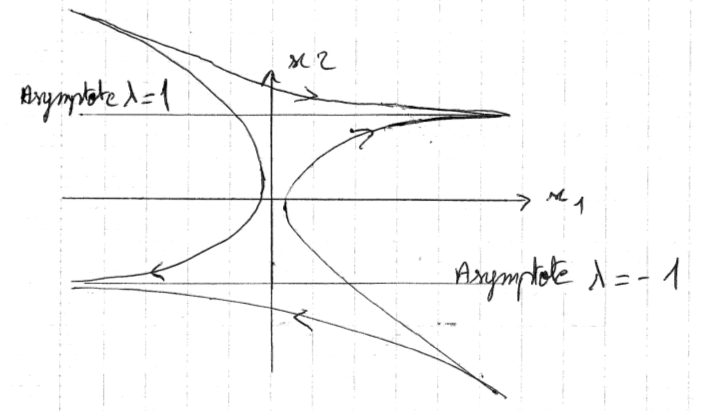
\includegraphics[width=0.9\textwidth]{1}
  \caption{ }
  \label{fig:label}
\end{figure}

\newpage
On a en sortie du comparateur: $\epsilon = x_1 + \beta x_2$
Sachant que l'on a la caractéristique: (attention, on a permuté avec $-R(\epsilon)$
\begin{figure}[ht]
  \centering
  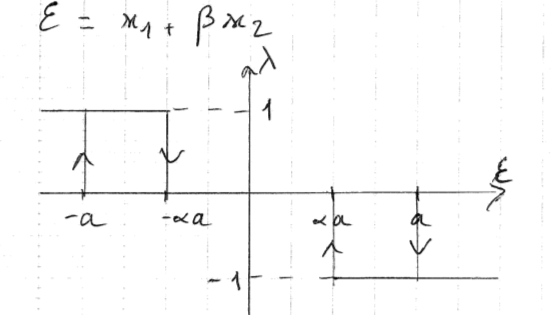
\includegraphics[width=0.9\textwidth]{2}
  \caption{ }
  \label{fig:label}
\end{figure}
On en déduit que:
\begin{figure}[ht]
  \centering
  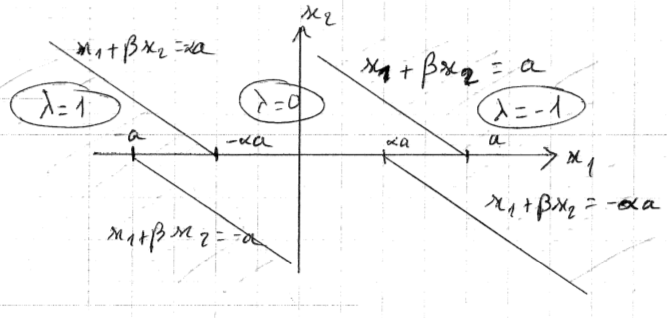
\includegraphics[width=0.9\textwidth]{3}
  \caption{ }
  \label{fig:label}
\end{figure}

Ainsi, selon la où l'on est, on va avoir différent $\lambda$, et on va pouvoir recouper ce graph avec celui de l'espace de phase précédent pour avoir le comportement du système dans l'espace de phase.
On parcourt donc l'espace de phase en partant du point P, puis on se déplace vers le point Q par la droite de pente -1, puis de Q a R et S pour revenir vers T sur la portion de courbe ou se situe P.
\begin{figure}[ht]
  \centering
  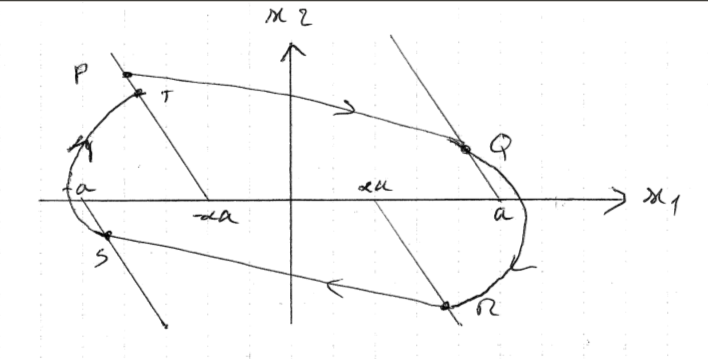
\includegraphics[width=0.9\textwidth]{4}
  \caption{ }
  \label{fig:label}
\end{figure}
Si $x_{2T} < x_{2P}$, alors on a stabilité et on converge vers le point d'équilibre 0.\\
Si $x_{2T} > x_{2P}$, alors on a un comportement instable et le système diverge.\\
Si $x_{2T} = x_{2P}$, alors on est sur le cycle limite.\\

\item On étudie chaque portion du cycle.

Entre le point P et Q on a comme relation:
\begin{align*}
x_{1p} + \beta x_{2p} & = -\alpha a\\
x_{1q} + \beta x_{2q} & = a
x_{1p} + x_{2p} & = x_{1q} + x_{2q} \text{	(dynamique)}
\end{align*}

Entre le point Q et R on a comme relation:
\begin{align*}
x_{1q} + \beta x_{2q} & = a\\
x_{1r} + \beta x_{2r} & = \alpha a\\
x_{1r} + x_{2r} & = x_{1q} + x_{2q} - ln\left(\frac{1+x_{2q}}{1+x_{2r}}\right) \text{	(dynamique)}
\end{align*}

Par symétrie, l'obtention du cycle limite vérifie $x_{2r} = -x_{2p}$. On a donc donc 6 inconnu et  6 équations différentes.

Ainsi, pour imposer le comportement du système, on fixe un cycle limite et l'on impose les valeurs de $a$ et $\alpha$ pour l'obtenir.
\end{enumerate}


\end{document}
